\documentclass[openany]{ctexart}
\usepackage{amssymb}
\usepackage{amsmath}
\usepackage{geometry} % 控制页面缩放
\usepackage{physics} % 一些方便的命令
\usepackage{booktabs} % 提供\toprule, \bottomrule
\usepackage{float} % 控制浮动体
\usepackage{subcaption} % 子图
\usepackage{fontspec} % 字体选择
\setmonofont{Consolas} % 设置无衬线字体为Consolas
\usepackage[T1]{fontenc} 
\usepackage{mathpazo} % 设置Palatino风格的西文字体
\usepackage{graphicx} 
\usepackage{enumitem} % 调整列表环境
\usepackage{abstract} % 调整摘要样式
\usepackage{bm}
\usepackage{listings,matlab-prettifier} % MATLAB代码美化包
\usepackage{CJK} %悬挂缩进
%\usepackage{enumitem} %条目行间距全局调整
%\setenumerate[1]{itemsep=0pt,partopsep=0pt,parsep=\parskip,topsep=0pt}
%\setitemize[1]{itemsep=0pt,partopsep=0pt,parsep=\parskip,topsep=0pt}
\lstset{
	style=Matlab-editor, numbers = left, numberstyle = \small, frame = single, basicstyle = \ttfamily
}
% 算法环境
\usepackage{algorithm}  
\usepackage{algorithmicx}  
\usepackage{algpseudocode}
\usepackage[hidelinks]{hyperref} % 引入交叉引用
\renewcommand{\abstractnamefont}{\heiti} % 摘要标题设置为黑体
% 对列表环境的设置
\setenumerate[1]{itemsep=0pt,partopsep=0pt,parsep=\parskip,topsep=5pt,listparindent=0em}
\setitemize[1]{itemsep=0pt,partopsep=0pt,parsep=\parskip,topsep=5pt,listparindent=0em}
\numberwithin{equation}{section} % 公式编号依照section
\geometry{a4paper,scale=0.8} % 内容占页面0.8
\def\celsius{\ensuremath{^\circ\hspace{-0.05em}\mathrm{C}}} % 定义摄氏度样式
\setcounter{tocdepth}{2} % 目录深度为2
% 设置致谢
\newcommand\Acknowledgements{\setcounter{secnumdepth}{-2}}

% xelatex --synctex=1 main.tex
\begin{document}

\title{\heiti 压水堆燃料管理与优化复习笔记}

\author{史锦康}

\date{\zhtoday}

\maketitle

%\begin{abstract}
%    这是摘要。
%    \par\noindent{\heiti 关键词:}关键词1;关键词2
%\end{abstract}

\newpage
%\tableofcontents
%
%\newpage

%% 正文部分 %%

\section{绪论(反应堆物理)}
\subsection{名词解释}

核反应堆:是指能以可控方式实现自持的链式裂变反应或核聚变反应的装置

易裂变核素:任意能量的中子都可引发其裂变,如:U-235、U-233、Pu-239

辐射俘获(n,$\gamma$):
$ _{92}^{235}U +_{0}^{1}n \longrightarrow  (_{92}^{236}U)^{*} \longrightarrow  _{92}^{236}U+\gamma$

裂变反应(n,f): 
$ _{92}^{235}U +_{0}^{1}n \longrightarrow  (_{92}^{236}U)^{*} \longrightarrow  _{Z1}^{A1}X +  _{Z2}^{A2}Y  + \upsilon_{0}^{1}n +200Mev $

可裂变核素:裂变反应具有阈能特点,只有快中子才能引起其裂变。Th-232、U-238、Pu-240

可转换核素:俘获一个中子后可经历一系列衰变成为易裂变核素的核素

剩余反应性:堆芯内没有任何毒物时所具有的反应性

换料周期: 反应堆两次停堆换料之间的时间间隔

循环长度: 一次装料后,反应堆能满功率运行的时间(有效满功率
天,EFPD)

%$ EFPD=\dfrac{一个循环内输出总能量}{堆芯名义功率}$

燃耗深度: \hspace{0.11111em}
\begin{minipage}[t]{\linewidth}
	装入堆芯的单位重量核燃料所产生的总能量的一种度
量,也是燃料贫化程度的一种度量.\newline(MW·d/kgU, GW·d/tU)
\end{minipage}
\vspace{0.05ex}

卸料燃耗:\hspace{0.11111em}
\begin{minipage}[t]{\linewidth}
	从堆芯中卸出的燃料所达的燃耗深度(受燃料元件材料性能限制,目前UO2燃料最大卸\newline 料燃耗深度在50~55 GW·d/tU)
\end{minipage}
\vspace{0.005ex}


分批换料:\hspace{0.11111em}
\begin{minipage}[t]{\linewidth}
	即在每次换料时,往往只将燃耗较深的那部分燃料卸出
	堆芯,而其余燃耗较浅的燃料则
	
	继续停留在堆内进行下一循环的
	运行。
\end{minipage}
\vspace{0.05cm}

循环燃耗:全堆芯所有的核燃料在经历了一个堆芯运行循环后所
净增的平均燃耗深度称为循环燃耗。

平均卸料燃耗深度: \hspace{0.11111em}
\begin{minipage}[t]{\linewidth}
	同一批卸出堆芯的燃料所具有的卸料燃耗
	平均值,它表征了这一批燃料所产生
	
	的能量,直接关系到反应堆
	的经济性
\end{minipage}
\vspace{0.005ex}


\subsection{问答题}

\begin{itemize}
	\item[1.] 堆内燃料管理的主要任务是什么?(经济性和安全性)\newline
	在满足电力需求和核燃料资源结构的约束,在电厂设计规范和技术要求的限制下,为核电厂一系列的运行循环做出满足经济性和安全性的全部堆芯换料决策。
	
	\vspace{1.5ex}
	
	\item[2.] 核电厂堆芯燃料管理的核心问题是什么?\newline
	在保证堆芯安全运行的条件下,单位发电成本最小化。
	
	\vspace{1.5ex}
	
	\item[3.] 堆芯燃料管理三阶段工作
	\begin{itemize}
		\item[a] 初步堆芯燃料管理策略及换料方案
		\item[b] 最终换料堆芯的全面核设计
		\item[c] 换料堆芯的安全评价
	\end{itemize}
	
\end{itemize}

\vspace{1.2ex}
\newpage

\section{核燃料循环概论}
\subsection{名词解释}
燃料管理:对整个核燃料循环提出安全经济的管理策略(堆前、堆内、堆后)

核燃料转换:通过中子俘获,将可裂变核素转换成易裂变核素(铀-钚循环、钍-铀循环)

转换比(CR):\hspace{0.11111em}
\begin{minipage}[t]{\linewidth}
核反应堆中每消耗一个易裂变材料原子所产生的新的易裂变材料原子数\newline
(当CR>1时,称为增殖比BR)
\end{minipage}
\vspace{0.05cm}

嬗变:\hspace{0.11111em}
\begin{minipage}[t]{\linewidth}
	通过中子俘获或裂变反应,把长寿命高放同位素转化为短寿命或稳定同位素
\end{minipage}

\subsection{问答题}
\begin{itemize}
	\item [1.] 为什么快中子反应堆更容易实现增殖?\newline
		对于$^{235}U$和$^{239}Pu$,只有在能量相当高的能区内,有效裂变中子数$\eta$才比2大得多,
		所以快堆内中子能谱愈硬(即中子平均能量越高),增殖性能就越好。
		
	\vspace{1.5ex}
	
	\item [2.] 常见的核燃料循环形式有哪些?
	\begin{itemize}
		\item [a.]一次性通过燃料循环
		\item [b.]回收铀循环(轻水堆)
		\item [c.]燃料增殖循环
		\item [d.]燃料联合循环
	\end{itemize}
	
	\item [3.]画出回收铀循环流程图\newline
	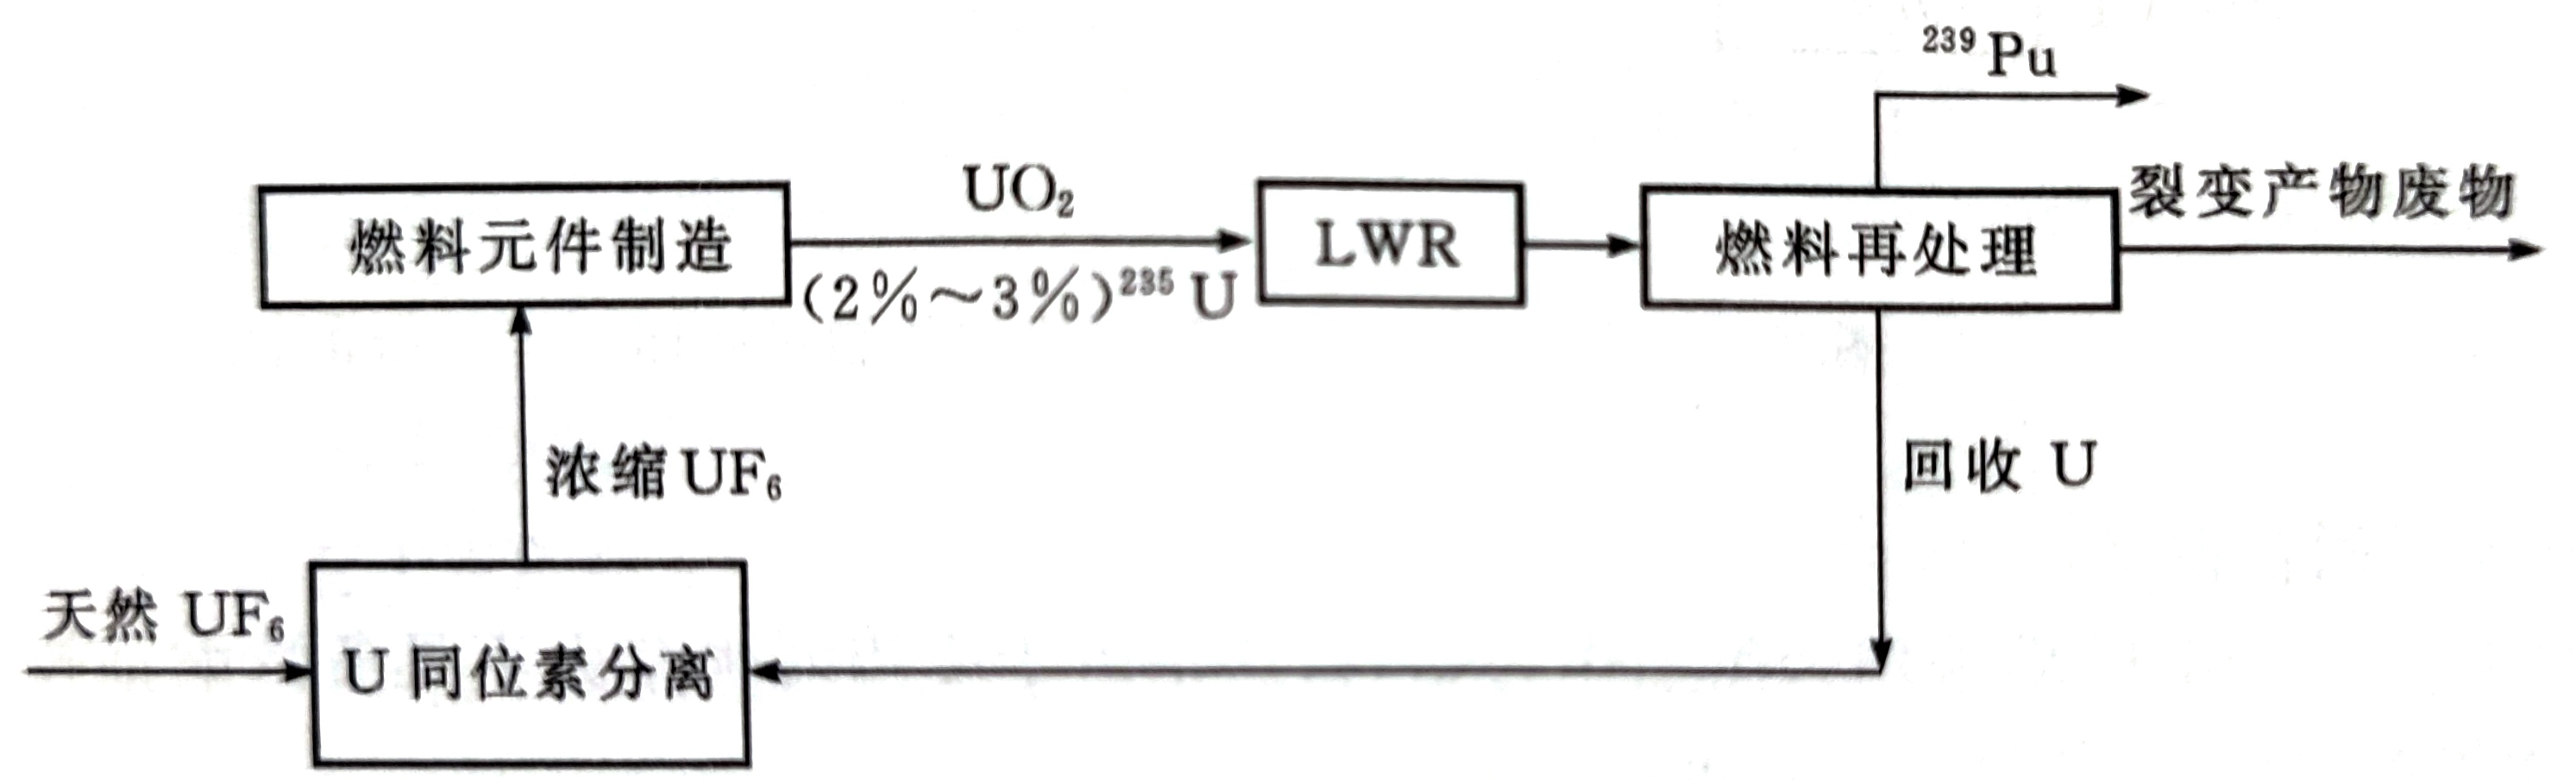
\includegraphics[width=10cm]{resource/lwr.jpg}
	\item [4.]画出铀-钚循环和钍-铀循环流程图\newline
	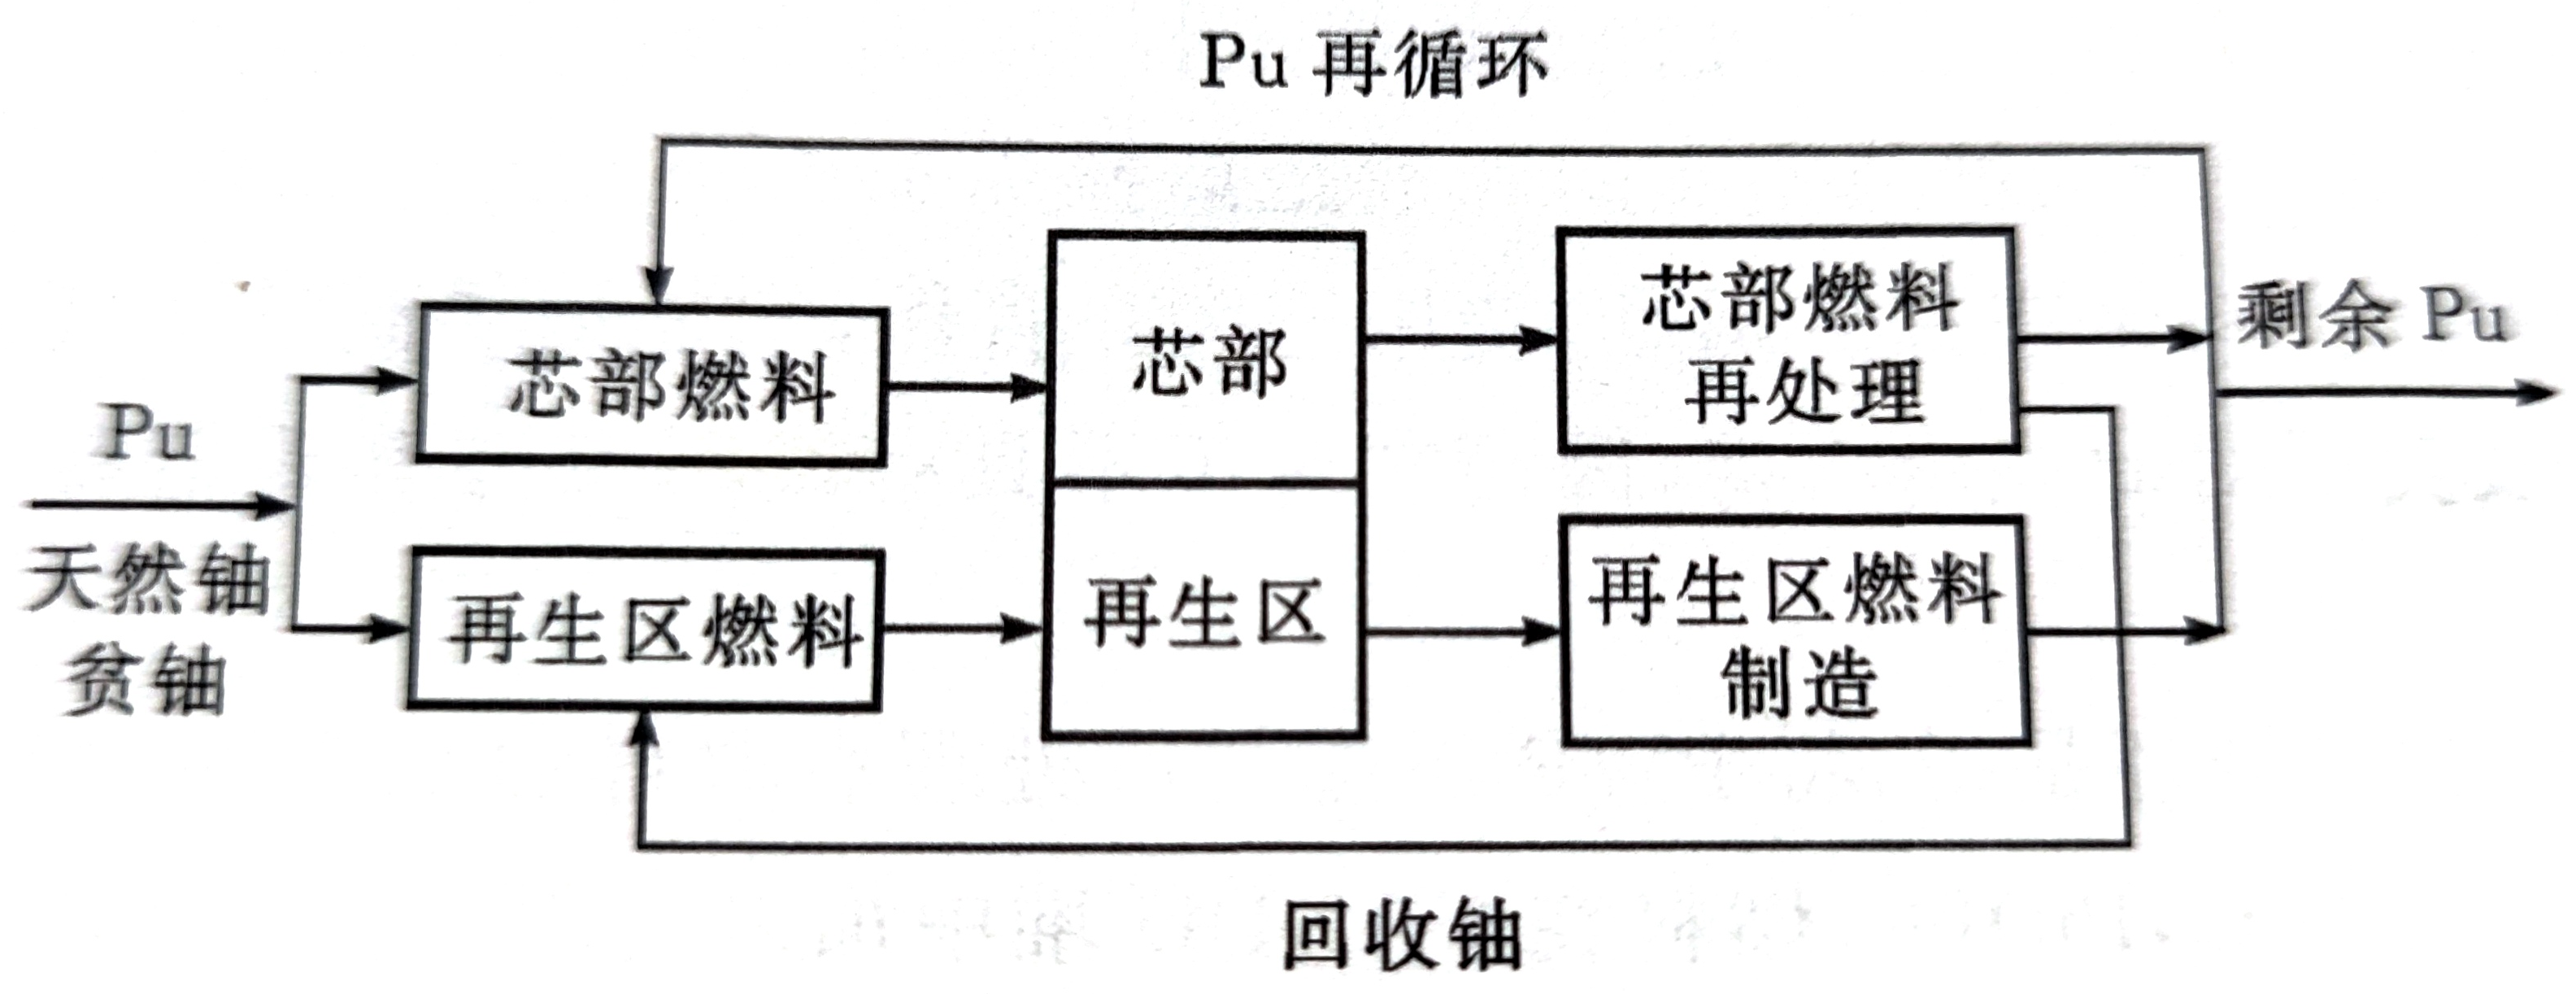
\includegraphics[width=10cm]{resource/upu.jpg}\newline
	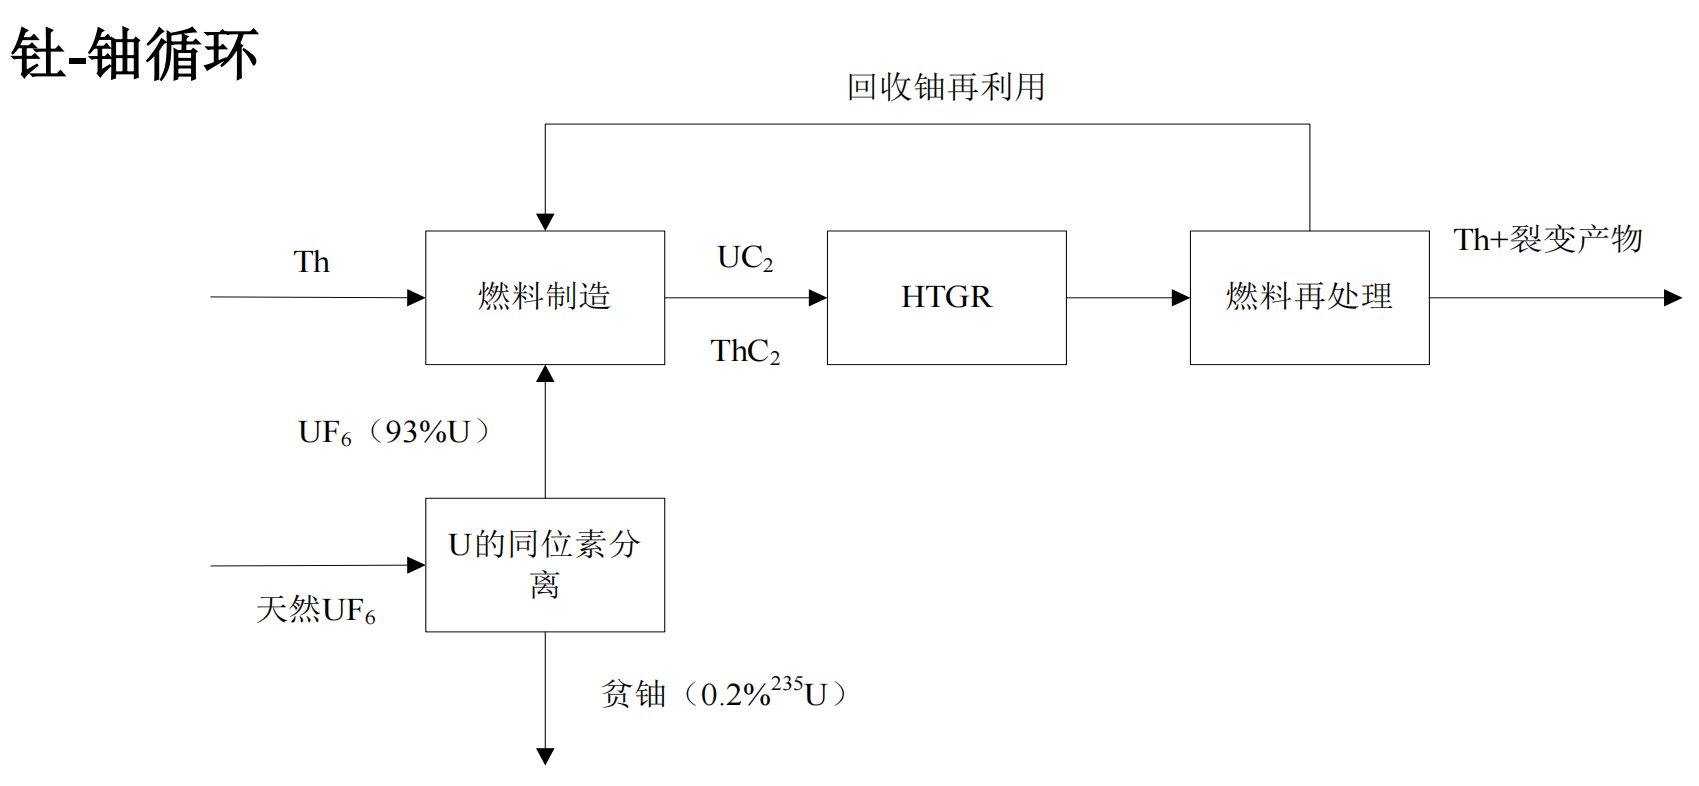
\includegraphics[width=7cm]{resource/tuu.png}

\end{itemize}

\newpage

\section{多循环燃料管理与优化}
\subsection{名词解释}
初始循环:反应堆首次启动运行的第一个循环,堆芯全部由新燃料组成。

过渡循环:从第2循环或扰动循环开始一直延续到平衡循环为止的各个循环。

平衡循环:\hspace{0.11111em}
\begin{minipage}[t]{\linewidth}
	每个循环的性能参数(如循环长度、新料富集度、一批换料量及平均卸料燃耗等)都保\newline
	持相同,运行循环到一个平衡状态。
\end{minipage}
\vspace{0.03cm}

扰动循环:\hspace{0.11111em}
\begin{minipage}[t]{\linewidth}
	是指由于燃料棒破损等原因导致平衡循环被破坏,直至新的平衡循环建立前的所有循环。
\end{minipage}
\vspace{0.05cm}

点堆分析模型:不考虑堆内的空间分布效应,燃料组件在堆内的空间影响仅以“批”考虑。

\subsection{问答题}
\begin{itemize}
	\item [1.] 给定燃料组件初始富集度$\epsilon$的情况下,换料批数n、与循环燃耗$B^c_{n}$、卸料燃耗$B^d_{n}$的关系($\alpha$为组件反应性随燃耗变化斜率,$\rho _{0}$为燃料组件初始反应性)\newline
	\begin{equation}
 		\large	B^d_{1}=\dfrac{\rho _{0}}{\alpha}
		\hspace*{1cm}
		\dfrac{B^d_{n}}{B^d_{1}}=\dfrac{2n}{n+1}
		\hspace*{1cm}
		\dfrac{B^c_{n}}{B^c_{1}}=\dfrac{2}{n+1}
	\end{equation}
	在线换料: $n \to \infty$
	
	\vspace{0.15cm}
	
	\item [2.]给定循环燃耗$B^c_{n}$的情况下,n批换料时寿期初堆芯的反应性:
	\begin{equation}
		\large \rho _{0,n} = \dfrac{n+1}{2} \alpha B^c_{n} = \dfrac{n+1}{2} \rho _{0,1}
	\end{equation}
	
	燃料组件初始反应性$\rho _{0}$和富集度$\epsilon$的关系
	\begin{equation}
		\large \rho _{0} \approx 0.1(\epsilon - 1.0\%)
	\end{equation}
	在保持平衡循环的循环燃耗不变的前提下,增加换料批次等于加深卸料燃耗,故新料富集度需提升。
	
	\vspace{0.15cm}
	
	\item [3.]在给定卸料燃耗的情况下,新燃料组件初始反应性随批料数变化的关系
	\begin{equation}
		\large \rho _{0,n} = \dfrac{n+1}{2n} \rho _{0,1}
	\end{equation}
	卸料燃耗给定的情况下,换料批次增加,可降低新料初始反应性(降低新料初始富集度)
	
	\vspace{0.15cm}
	
	\item  [4.]向平衡循环过渡的三种方式
	\begin{itemize}
		\vspace{-0.01cm}
		\item  [a.]固定循环燃耗及一批换料量,调节新料富集度
		\vspace{-0.01cm}
			\item  [b.]固定循环燃耗及新料富集度,调节一批换料量
			\vspace{-0.01cm}
				\item  [c.]固定新料富集度及一批换料量,调节循环燃耗
	\end{itemize}
	
\end{itemize}

\newpage

\section{单循环燃料管理与优化}
\subsection{名词解释}
堆芯换料优化:\hspace{0.11111em}
\begin{minipage}[t]{\linewidth}
	通过寻求满足约束条件的最优布料方案和可燃毒物布置方案,来达到最安全或最经\newline
	济的目标(安全性:功率峰因子最小;经济性:组件平均卸料燃耗增加)
\end{minipage}
\vspace{0.03cm}

功率峰因子:最大功率密度和平均功率密度的比值。

剩余反应性:堆芯没有任何毒物时的反应性。

可燃毒物的反应性惩罚:可燃毒物的存在导致反应堆寿期缩短的部分。

临界硼浓度:\hspace{0.11111em}
\begin{minipage}[t]{\linewidth}
   某一燃耗时刻,不考虑控制棒,完全用堆芯中的可燃毒物和可溶硼来控制,使得核反应堆处于临界所需要的硼浓度
\end{minipage}
\vspace{0.03cm}

\subsection{问答题}
\begin{itemize}
	\item [1.]  {\heiti Out-In装载方案}
	\vspace{-0.08cm}
	\begin{itemize}
		\item [优点:]
		\begin{itemize}
			\item [a.]展平全堆中子通量分布、降低整体功率峰。
			\item [b.]降低局部功率峰因子。
		\end{itemize}
		\item [缺点:]
		\begin{itemize}
			\item [a.]中子泄露比较严重,导致中子利用率降低以及对压力壳的辐照严重。
		\end{itemize}
	\end{itemize}
	
	\vspace{0.06cm}
	
	\item [2.]{\heiti 低泄漏装载方案}
	\vspace{-0.08cm}
	\begin{itemize}
		\item [优点:]
		\begin{itemize}
			\item [a.]减少了中子从堆芯的泄漏,提高了中子利用的经济性,延长了堆芯寿期
			\item [b.]在给定循环长度和新料组件数的情况下,降低燃料富集度
			\item [c.]对压力壳的辐照损伤小,延长反应堆实用寿命
		\end{itemize}
		
		\item [缺点:]
		\begin{itemize}
			\item [a.]功率峰值增加,堆芯需要布置可燃毒物,存在可燃毒物反应性惩罚
			\item [b.]堆芯设计难度增加
		\end{itemize}
	\end{itemize}
	
	\vspace{0.06cm}
	
	\item [3.]{\heiti 换料设计优化常用的约束条件}
	\vspace{-0.06cm}
	\begin{itemize}
		\item [a.]整个循环的最大功率峰因子小于许可值
		\item [b.]燃料组件的最大卸料燃耗小于许可值
		\item [c.]堆芯慢化剂温度系数为负值
		\item [d.]停堆深度不低于某一定值
		\item [e.]新料富集度小于规定值
	\end{itemize}
	
		\vspace{0.06cm}
		
	\item [3.]{\heiti 堆芯换料优化常用模型}
	\vspace{-0.08cm}
	\begin{itemize}
		\item [a.]专家系统
		\item [b.]遗传算法(GA)
		\item [c.]模拟退火算法(SA)
		\item [d.]神经网络算法
	\end{itemize}
\end{itemize}

\section{单循环燃料管理计算}
\subsection{精华}

    {\centering 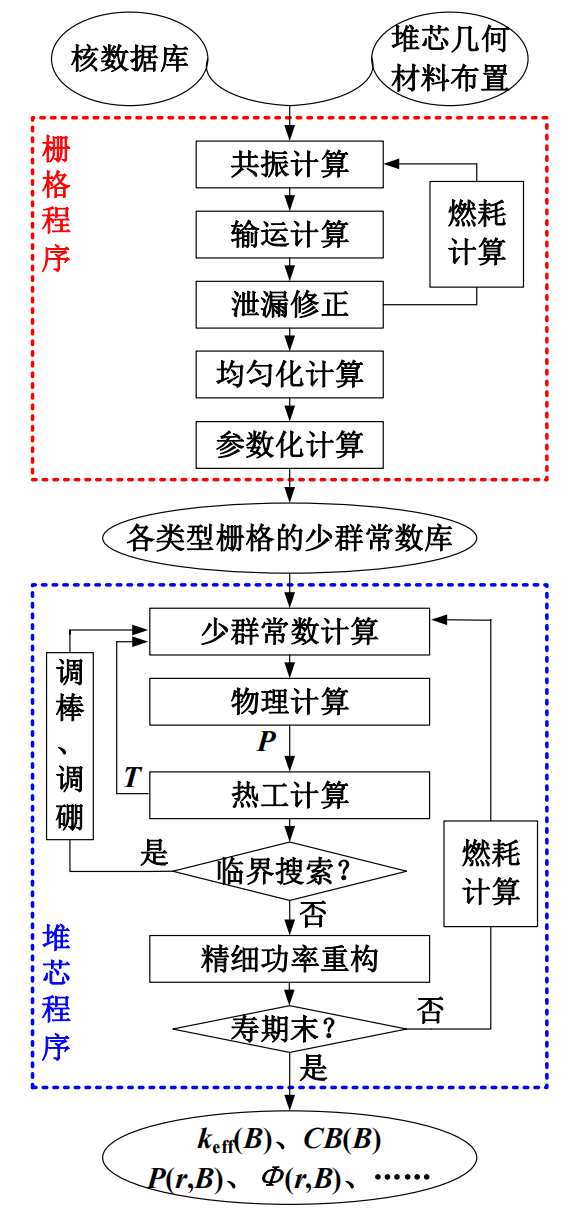
\includegraphics[width=10cm]{resource/5-1.png}}
%	\newpage
\subsection{知识要点}
\begin{itemize}
	\item [1.]两步法 = 栅格计算+堆芯计算 \hspace*{0.3cm}(核心思想:分步均匀化)
	\item [2.]核数据处理的任务:将评价库中的核数据转化为中子学软件所需的专门数据库
	\item [3.]栅格共振计算:求解多群输运方程时,需要多群截面。采用反应率守恒原则,以中子能谱为权重,计算多群平均截面。
	\begin{equation}
	\Large	\sigma _{x,g}^{eff} = \dfrac{\int_{\Delta E_{g}} \sigma _{x}(E) \phi (E) dE}{\int_{\Delta E_{g}} \phi (E) dE}
	\end{equation}
	
	\item [4.]共振计算的目的:得到共振核素在实际问题中共振能群的有效自屛截面(共振能群的平均截面),为多群输运求解提供截面参数。
	\item [5.]共振计算方法
	\begin{table}[!ht]
		\centering
		\begin{tabular}{|l|l|l|l|}
			\hline
			方法 &  几何适应性 & 核心计算 & 效率 \\ \hline
			等价理论 & 简单规则几何 & 有理近似参数, 等效稀释截面 & 1(高) \\ \hline
			子群、概率表、多邦 & 取决于中子输运计算 & 子群参数、子群中子能谱 & 2 \\ \hline
			超细群 &  多种规则几何 & 超细群中子能谱 & 3 \\ \hline
			连续能量 & 取决于中子输运计算 &  连续中子能谱展开系数 & 4 \\ \hline
		\end{tabular}
	\end{table}
	
	\item [6.]栅格输运计算:在共振计算给出共振能群的有效截面后,整个二维栅格内所有区域所有能群的中子核反应截面都是已知的,就可以在整个二维栅格范围内进行栅格输运计算,获得非均匀栅格内的中子通量分布,如果是燃料栅格还会获得其无限增殖因子。\\
	常用的输运方法
		\vspace{-0.08cm}
	\begin{itemize}
		\item [a.]离散纵标方法(Sn)
		\vspace{-0.08cm}
			\item [b.]球谐函数方法(Pn)
			\vspace{-0.08cm}
				\item [c.]特征线方法(MOC)
				\vspace{-0.08cm}
					\item [d.]碰撞概论方法(CPM)
	\end{itemize}
	\vspace{0.1cm}
	\item [7.] 泄漏修正:由于组件输运计算的时候通常是二维的,四周为全反射边界条件,即无
	限介质栅格,也就是说没有考虑中子泄漏,而燃料组件在真实堆芯中存在泄漏,所
	以需要对燃料组件输运计算得到的通量进行修正以考虑泄漏的影响,这种做法通常
	被称为泄漏修正。
	
	\vspace{0.12cm}
	
	\item [8.]预估校正法:即先根据当前燃耗步初始时刻的原子核密度进行中子学计算 (求解中子输运方程)得到初始时刻的微观反应率,然后用该反应率求解当前燃耗步长内的燃耗方程得到燃耗步长末的原子核密度,称为预估步的原子核密度,然后用预估步的原子核密度再求解一次中子学计算得到步长末的微观反应率,用该微观反应率再求解一次当前燃耗步的燃耗方程,得到燃耗步长末的原子核密度,称为校正步的原子核密度。
	
	\vspace{0.1cm}
	
	\item [9.] 组件均匀化三个守恒原则
		\begin{itemize}
			\item [a.]所有群的反应率守恒
			\vspace{-0.08cm}
			\item [a.]节快的各个界面上的界面净流守恒
			\vspace{-0.08cm}
			\item [a.]反应堆的特征值守恒
			\vspace{-0.08cm}
		\end{itemize}
	
\end{itemize}


\section{堆芯核设计}
\subsection{名词解释}
\begin{itemize}
	
\item [1.]轴向功率偏移(AO):堆芯上部功率$P_{H}$和下部功率$P_{B}$之差除以堆芯功率。
\begin{equation}
	\Large AO=\dfrac{P_{H}-P_{B}}{P_{H}+P_{B}} \times 100\%
\end{equation}
{\heiti 常轴向偏移控制:} 反应堆正常运行时,要求不管运行功率水平是多少,要求保持同样的轴向功率分布形状,用轴向功率偏移$ AO=AO_{ref}$ 来控制反应堆

\vspace{0.1cm}

\item [2.]轴向功率偏差 $\Delta I$ :堆芯上部和下部功率差值。
\begin{equation}
   \Large  \Delta I = P_{H}-P_{B}
\end{equation}

\item [3.]慢化剂温度系数:慢化剂平均温度每变化1K引起的堆芯反应性变化。
\item [4.]多普勒功率系数:功率每变化额定功率的1\% 时由多普勒效应引起的反应性变化。
\item [5.]功率系数:堆芯功率每变化额定功率的1\% 时由慢化剂和燃料温度效应共同引起的反应性变化。
\item [6.]硼微分价值:堆芯单位硼浓度变化引起的反应性变化。
\item [7.] 压水堆三种控制方式:可溶硼、可燃毒物、控制棒。
\item [8.]停堆裕量:堆芯临界运行条件下,考虑了堆芯功率降低引入的正反应性和最大价值的一束控制棒卡在高位的情况,其他控制棒插入后反应堆将达到的次临界水平。
\item [9.]停堆深度:将控制毒物全部投入堆芯产生的次临界度。
\item [10.]控制棒咬量:主调节棒组的最小插入深度。
\item [11.]控制棒插入极限:控制棒插入的最大深度。
\item [12.]首次启动物理试验:首次临界、零功率物理试验和升功率过程在各功率台阶上的物理试验。
\end{itemize}



\subsection{知识点}
\begin{itemize}
	\item [1.]堆芯核设计主要任务:从反应堆物理角度,以应用层面指导核电厂运行。
			\vspace{0.08cm}
	\item [2.]核电厂堆芯核设计主要内容:
	\begin{itemize}
		\vspace{-0.12cm}
		\item [a.]堆芯燃耗和燃料管理
		\vspace{-0.15cm}
		\item [b.]堆芯功率能力
		\vspace{-0.15cm}
		\item [c.]反应性控制
		\vspace{-0.15cm}
		\item [d.]反应性系数
		\vspace{-0.15cm}
		\item [e.]中子源
	\end{itemize}
	
	\item [3.]堆芯燃耗和燃料管理分析的目的
	\begin{itemize}
		\vspace{-0.1cm}
		\item [a.]确保第一循环到平衡循环燃料管理方案技术上可行
		\vspace{-0.15cm}
		\item [b.]为热工水力分析、燃料性能分析、堆芯功率能力和反应性控制提供参数
		\vspace{-0.15cm}
		\item [c.]为安全分析报告(FSAR)提供基础数据
	\end{itemize}
\end{itemize}


\newpage

\section{换料堆芯安全评价}
\subsection{知识点}
\begin{itemize}
	\item [1.]换料堆芯安全评价的基本原理和方法:{\heiti 安全边界分析法},其基本思想:
	\begin{itemize}
		\item [1)]对于给定的事故,当换料堆芯所有与事故有关的参数都保守地处于FSAR安全分析的边界限值以内,则FSAR的结论都是适用的,从而确认了该换料堆芯对给定事故的安全性。
		
		\item [2)]当换堆芯的关键安全参数超出FSAR的安全边界值,则需要对有关事故或换料堆芯进行重新分析或评价,以确定该超限参数对堆芯安全性的影响,必要时还需要修改相关的技术规格书和运行规程。
		
		\item [3)]如果重新分析和评价仍不能满足安全准则要求,则需要重新设计换料堆芯的装载方案以满足反应堆运行的安全需求。
		
	\end{itemize}
	
	\item [2.]关键安全参数:影响堆芯正常运行或瞬态特性,以及事故工况发展后果的物理和热工参数。
	
	\vspace{0.15cm}
	
	\item [3.]通用关键安全参数:对许多瞬态和事故发生影响的堆芯参数。
		\begin{itemize}
		\vspace{-0.1cm}
		\item [1)]慢化剂密度系数
		\vspace{-0.1cm}
		\item [2)]多普勒温度系数
		\vspace{-0.1cm}
		\item [3)]多普勒功率系数
		\vspace{-0.1cm}
		\item [4)]有效缓发中子份额
		\vspace{-0.1cm}
		\item [5)]最大微分棒价值
		\vspace{-0.1cm}
		\item [6)]最大瞬发中子寿命
		\vspace{-0.1cm}
		\item [7)]沿轴向归一化的最小停堆反应性引入
	\end{itemize}
	
	\vspace{0.15cm}
	
	\item [4.]代表性特定事故:
		\begin{itemize}
			\vspace{-0.1cm}
			\item [1)]不可控硼稀释事故
			\vspace{-0.1cm}
			\item [2)]提棒事故、落棒事故、弹棒事故
			\vspace{-0.1cm}
			\item [3)]主蒸汽管道断裂事故
			
		\end{itemize}
\end{itemize}

\end{document}